\chapter{Software Project Telemetry}
\label{Chapter:Telemetry}


Software project telemetry is a novel, light-weight, and extensible software measurement approach proposed in this thesis. It includes both (1) highly automated measurement machinery for metrics collection and analysis, and (2) a methodology for in-process, empirically-guided software development process problem detection and diagnosis. In this approach, sensors collect software metrics automatically and unobtrusively. Metrics are abstracted in real time to telemetry streams, charts, and reports, which represent high-level perspectives on software development. Telemetry trends are the basis for decision-making in project management and process improvement. Unlike traditional approaches which are primarily based on historical project database and focused on comparison of similar projects, software project telemetry focuses on project dynamics and in-process control. It combines both the precision of traditional project management techniques and the flexibility promoted by agile community.

This chapter is organized into the following sections. 
Section \ref{Telemetry:Overview} gives an overview of software project 
        telemetry and its essential characteristics.
Section \ref{Telemetry:Data} discusses sensor-based metrics 
        collection. 
Section \ref{Telemetry:Component} discusses telemetry streams, 
        charts, and reports, which capture high-level perspectives on software development.
Section \ref{Telemetry:Language} discusses the telemetry language, which
        provides a flexible mechanism to construct telemetry streams, charts, 
        and reports, and which facilitates interactive exploration of different perspectives 
        on software development.
Section \ref{Telemetry:Process} discusses the telemetry-based methodology for 
        project management and process improvement.
%Section \ref{Telemetry:Example} gives an example to illustrate how software
%        project telemetry works. 
Section \ref{Telemetry:Conclusion} summarizes this chapter.





%Software project telemetry works seamlessly with the existing GQM paradigm and maturity-based frameworks to improve the capability of software development organizations by supplementing them with an explicit and practical framework for metrics collection and analysis. It also addresses the cost problem of measurement programs by completely automating the measurement process.


%%%%%%%%%%%%%%%%%%%%%%%%%%%%%%%%%%%%%%%%%%%%%%%%%%%%%%%%%%%%%%%%%%%%%%%%%%%%%%%%%%%%%%%
%%%%%%%%%%%%%%%%%%%%%%%%%%%%%%%%%%%%%%%%%%%%%%%%%%%%%%%%%%%%%%%%%%%%%%%%%%%%%%%%%%%%%%%

\section{Overview} 
\label{Telemetry:Overview}

%\textcolor{red}{[Ask Philip how to deal with material copied from 04-11.]}

\textit{Encyclopedia Britannica} defines telemetry as \textit{``highly automated communication process by which data are collected from instruments located at remote or inaccessible points and transmitted to receiving equipment for measurement, monitoring, display, and recording''}. Perhaps the highest profile user of telemetry is NASA, where telemetry has been used since 1965 to monitor space flights staring from the early Gemini missions to the modern Mars rover flights. Telemetry data, collected by sensors attached to a space vehicle and its occupants, are used for many purposes, such as gaining better insight into mission status, detecting early signals of anomalies, and analyzing impacts of mission adjustments.

Applying this concept to software project management, I define \textit{software project telemetry} as an automated software process and product measurement approach. In this approach, sensors unobtrusively collect time-stamped software metrics, which are abstracted into telemetry streams in real time. Telemetry streams are the basis for project management and process improvement. Telemetry charts and reports provide visualization. By detecting changes and covariance among different telemetry streams, software project telemetry enables a more incremental, visible, and experiential approach to project decision-making. It has both the precision of traditional project management techniques and the flexibility promoted by agile community.

Software project telemetry has following essential characteristics:

%\begin{itemize}
%  \item Software metrics are collected automatically and unobtrusively by sensors.
%  \item Software telemetry streams are made from time-stamped metrics, and updated in real time.
%  \item Telemetry streams serve as the basis for software project monitoring and control, as well as process improvement hypothesis validation. 
%  \item Software metrics are always time-stamped, software telemetry streams are made from time-stamped metrics, and time-stamp is significant for analysis.
%  \item Software telemetry streams are updated continuously, and immediately made available to both developers and managers.
%  \item Metrics analysis exhibits graceful degradation in case of missing data.
%  \item Software project telemetry is used for in-process monitoring and control.
%\end{itemize}


\begin{enumerate}
\item \textit{Software project telemetry data is collected automatically by tools
   that unobtrusively monitor some form of state in the project
   development environment.}  In other words, software developers are
   working in a ``remote or inaccessible location'' from the perspective of
   metrics collection activities. This contrasts with software metrics data
   that require human intervention or developer effort to collect, such as
   PSP/TSP metrics \cite{Humphrey:1995}.
\item \textit{Software project telemetry data consists of a stream of
   time-stamped events, where the time-stamp is significant for analysis.}
   Software project telemetry data is thus focused on evolutionary
   processes in development.  This contrasts, for example, with COCOMO
   \cite{Cocomo:1981, Cocomo:2000}, where the time at which the calibration data was
   collected about the project is not significant.
\item \textit{Software project telemetry data is continuously updated and immediately 
   available to both developers and managers.}  Telemetry data is not hidden
   away in some obscure database guarded by the software quality improvement
   group.  It is easily visible to all members of the project for 
   interpretation. 
\item \textit{Software project telemetry exhibits graceful degradation.}
   While complete telemetry data provide best support for project
   management, the analyses are not brittle: they still provide
   value even if complete sensor data are not available. For example, 
   telemetry analyses can still provide decision-making
   value even if data collection starts midway through a project.      
\item \textit{Software project telemetry is used for in-process monitoring,
   control, and short-term prediction.} Telemetry analyses provide
   representations of current project state and how it is changing at
   various time scales.  The simultaneous display of multiple project state values and
   how they change over the same time periods allow opportunistic
   analyses --- the emergent knowledge that one state variable appears to
   co-vary with another in the context of the current project.
\end{enumerate}




%%%%%%%%%%%%%%%%%%%%%%%%%%%%%%%%%%%%%%%%%%%%%%%%%%%%%%%%%%%%%%%%%%%%%%%%%%%%%%%%%%%%%%%
%%%%%%%%%%%%%%%%%%%%%%%%%%%%%%%%%%%%%%%%%%%%%%%%%%%%%%%%%%%%%%%%%%%%%%%%%%%%%%%%%%%%%%%

\section{Sensor-based Data Collection}
\label{Telemetry:Data}


%Software measurement and metrics collection is always at the core of software process improvement programs. Measurement capability determines, to a large extent, whether any process improvement initiatives can be successfully implemented or not in a software organization. It's important that metrics be collected in a cost-effective way, and both the management and developers are convinced of usefulness of software measurement. However software measurement can be expensive, especially when done on a continual basis. Few organizations can afford to apply measurement to all development activities and products to get a comprehensive quantitative view. 

In software project telemetry, software metrics are collected \textit{automatically} by sensors that \textit{unobtrusively} monitor some form of state in the project development environment. Sensors are pieces of software, and they collect both \textit{process} and \textit{product} metrics.

Sensors collecting process metrics are typically implemented in the form of plug-ins, which are attached to software development tools in order to continuously monitor and record their activities in the background. Some examples are listed below:

\begin{itemize}

	\item A plug-in for an IDE (integrated development environment) such as Visual Studio \cite{Software:VisualStudio}, and Eclipse \cite{Software:Eclipse}. It can record individual developer activities automatically and transparently, such as code editing effort, compilation attempts and results, etc.

  \item A plug-in for a version control system, such as Rational Clear Case \cite{Software:ClearCase}, and CVS \cite{Software:CVS}. It can monitor code check-in and check-out activities, and compute \textit{diff} information between different revisions.
  
  \item A plug-in for a bug tracking or issue management system, such as Bugzilla \cite{Software:Bugzilla}, and Jira \cite{Software:Jira}. Whenever an issue is reported or its status has changed, the sensor can detect such activities and record the relevant information.
  
  \item A plug-in for an automated build system, such as Cruise Control \cite{Software:CruiseControl}. It can capture information related to build attempts and build results.

\end{itemize}


Sensors collecting product metrics are typically implemented as automated analyzers for software artifacts. Typically, these analyzers need to be scheduled to run periodically in order to acquire the continual flow of metrics required by telemetry streams. To automate these tasks, one can use a \textit{Cron} job\footnote{\textit{Cron} is a \textit{Unix/Linux} program that enables users to execute commands or scripts automatically at a specified time or date. The \textit{Windows} equivalent is called \textit{Scheduled Tasks}.}, or run them as a task in some automated build system. Some examples are listed below:

\begin{itemize}

	\item An analyzer parsing program source code to compute size or complexity information.
	
	\item An analyzer to parse the output of coverage tools, such as Clover \cite{Software:Clover}, and JBlanket \cite{Software:JBlanket}, to retrieve testing coverage information.

\end{itemize}



There are many other possibilities. One can even imagine writing an exotic sensor that retrieves project cost information from company accounting database, if such information is useful and the practice is allowed by company policy. No matter what the sensor does and regardless of the implementation details, a sensor-based approach collects metrics unobtrusively in order to keep data collection overhead low, so that developers are not distracted from their primary tasks -- developing software products instead of capturing process and product metrics.


% Comparison of sensor data collection with other data collection techniques.

There is no chronic overhead in sensor-based metrics collection. Though setting up sensors requires effort, once they are installed and configured, sensor data collection is automatic and unobtrusive. This contrasts with traditional data collection techniques, such as paper-and-pencil based approach used in PSP/TSP \cite{Humphrey:1995}, or tool-supported approach used in LEAP \cite{Moore:1999}, PSP Studio \cite{PspStudio:1997}, and Software Process Dashboard \cite{PspDashboard:2000}, which require either human intervention or developer effort. Even in the case of tool-supported approach, the developer still bears the chronic overhead of constantly switching back and forth between doing work and telling the tool what work is being done \cite{Johnson:2001, Johnson:2003}.

The fact that chronic overhead is removed from sensor-based metrics collection not only reduces the adoption barrier of the technology, but also makes it feasible for software organizations to apply measurements to a wide range of development activities and products in order to get a comprehensive quantitative view of development processes.


% Restriion of sensor based data collection.

The sensor-based approach does impose some restrictions:

\begin{itemize}
	
	\item A sensor must be developed for each type of tool we wish to monitor. This is a one-time cost. Once the sensor is developed, it can be used by different software development organizations for different projects. The Collaborative Software Development Lab has already developed a repository of over 20 sensors for commonly-used tools.

  \item Some metrics may not be amenable to automated data collection. An example would be developer effort. While it is possible to instrument an IDE to automatically get information such as how many hours a developer has spent on writing code, it is almost impossible to construct a sensor that knows how much total effort a developer has contributed to a project. For instance, two developers might be discussing the design of a system in the hallway. It is very difficult to collect this type of effort automatically. It is still open research question whether all important metrics can be captured by sensors or not. This thesis takes a more pragmatic view, and is only concerned with whether sensors can collect sufficient metrics so that software project telemetry can deliver value to project management and process improvement. 
  
  %Sometimes, this is related to an organization's process maturity level. At low maturity level, process and artifacts are not not well-define. So hard to collect metrics mechanically. But the problem can be solved once the software organization matures. 
 
\end{itemize}


%The total cost of sensor-based approach is extremely low. Apart from one-time cost of developing custom sensors for the development tools we wish to monitor, there is no other cost since sensors work transparently and autonomously. The low cost of ownership 





%%%%%%%%%%%%%%%%%%%%%%%%%%%%%%%%%%%%%%%%%%%%%%%%%%%%%%%%%%%%%%%%%%%%%%%%%%%%%%%%%%%%%%%
%%%%%%%%%%%%%%%%%%%%%%%%%%%%%%%%%%%%%%%%%%%%%%%%%%%%%%%%%%%%%%%%%%%%%%%%%%%%%%%%%%%%%%%

\section{Telemetry Reducer, Stream, Chart, and Report} 
\label{Telemetry:Component}

A \textit{telemetry report} is a named set of telemetry charts that can be generated for a specified project over a specified time interval. The goal of a telemetry report is to discover how the trajectory of different process and product metrics might influence each other over time, and whether these influences change depending upon context.
A \textit{telemetry chart }is a named set of telemetry streams. The goal of a telemetry chart is to display the trajectory over time of one or more process or product metrics.
A \textit{telemetry stream} is a sequence of a single type of process or product data. Telemetry streams are best thought of as a kind of abstract data type representing one or more series of metric data values of a similar type. In addition, they support basic arithmetic operations. The details are discussed in Section \ref{Intro:Solution:MeasurementMachinery}. 
 
The data collected by sensors are time-stamped, and this time stamp is always significant in telemetry style metrics analysis. There may not be one-to-one correspondence between sensor data and the data points in the telemetry stream. Sensor data usually represents very fine-grained low level software process or product details, while the data points in the telemetry stream represent higher level perspectives on the software system. Typically, sensor data need to be filtered, combined, aggregated, or post-processed to derive a telemetry data point. This is the job of \textit{telemetry reducers}, which take sensor data as input, and output telemetry data points.

A \textit{telemetry reducer} serves as the bridge between \textit{sensor data} and \textit{telemetry stream}. For example, suppose we want to construct a telemetry stream representing the number of open bugs for a development project on a monthly interval for the entire year 2004. Suppose we are using Bugzilla \cite{Software:Bugzilla}, and a Bugzilla sensor has been installed since the start of the project. Suppose whenever a bug is opened or closed, the Bugzilla sensor records information such as event time stamp, event type (bug open or bug close), bug id, severity, etc. In order to compute the number of open bugs for each month in 2004, the telemetry reducer needs to scan the entire bug event sensor data.    

Telemetry reducer is the building block of telemetry stream. A reducer must be available in order to construct a ``simple'' telemetry stream\footnote{Telemetry streams can also be generated by applying mathematical operations to existing telemetry streams. These are called ``compound'' telemetry streams as opposed to ``simple'' telemetry streams. See Section \ref{Telemetry:Language} for details.}. Some example of general classes of software project telemetry are:

%\textit{Telemetry streams} consist of streams of time-stamped \textit{telemetry events}. Time-stamp is always significant in telemetry-based analysis. By their construction, software telemetry streams are focused on development dynamics and process change. The nature of telemetry streams makes them ideal for in-process monitoring and control. It also enables experimental approach to software project decision-making by allowing one to monitor the changes in telemetry streams for the impact of the decisions. 

%Telemetry streams are allowed to be combined as well to generate new telemetry streams revealing higher level information about software development process. 

%The update of telemetry streams is continuous. Whenever there is new sensor data, the relevant telemetry streams can be updated and immediately made available to both developers and managers. 

%The analysis based on software project telemetry is flexible. The types of metrics that can be collected is only constrained by the available of sensors. It is always possible to write a new sensor to collect new type of software metrics, and there is virtually limitless possibilities of generating telemetry streams by filtering, combining, and aggregating the metrics. 

%Telemetry analysis is robust. There is no requirement for complete set of telemetry data. While complete set of telemetry data provides best support for project management, the telemetry analysis can still provide value even if sensor data occasionally become unavailable.



\begin{itemize}
	\item \textit{Development Telemetry} --- These are telemetry streams generated from data gathered by observing the behavior of software developers as reflected in their tool usage, such as the information about the files they edit, the time they spend using various tools, and the changes they make to project artifacts, the sequences of tool or command invocations, and so forth. Such metrics can be collected by attaching sensors to Integrated Development Environments (e.g. Visual Studio, Eclipse, Emacs.), configuration management system (e.g. CVS \cite{Software:CVS}, Clear Case \cite{Software:ClearCase}.), issue management systems(e.g. Bugzilla \cite{Software:Bugzilla}, Jira \cite{Software:Jira}.), etc.
	
	\item \textit{Build Telemetry} --- These are telemetry streams generated from data gathered by observing the results of tools invoked to compile, link, and test the system. Such metrics can be collected by attaching sensors to build tools (e.g. Make, Ant \cite{Software:Ant}, Cruise Control \cite{Software:CruiseControl}.), testing tools(e.g. JUnit \cite{Software:JUnit}.), size and complexity counters(e.g. LOCC \cite{Software:LOCC}.), etc.
	
	\item \textit{Execution Telemetry} --- These are telemetry streams generated from data gathered by observing the behavior of the system as it executes. Such metrics can be collected by sensors attached to the system runtime environment to gather its internal state data (e.g. heap size, occurrence of exceptions.), or to load testing tools (e.g. JMeter \cite{Software:JMeter}) of the system to gather system performance data.
	
	\item \textit{Usage Telemetry} --- These are telemetry streams generated from data gathered by observing the behavior of users as they interact with the system, such as the frequency, types, and sequences of command invocations during a given period of time in a given system.

\end{itemize}



%\textit{Telemetry chart} and \textit{telemetry report} are visual representation of one or more telemetry streams for the same time period with the same interval scale. The basic idea behind them is that by juxtaposing different telemetry streams, it helps project manager to detect covariance between them. Section \ref{Intro:Solution:MeasurementMachinery} contains the detail.







%%%%%%%%%%%%%%%%%%%%%%%%%%%%%%%%%%%%%%%%%%%%%%%%%%%%%%%%%%%%%%%%%%%%%%%%%%%%%%%%%%%%%%%
%%%%%%%%%%%%%%%%%%%%%%%%%%%%%%%%%%%%%%%%%%%%%%%%%%%%%%%%%%%%%%%%%%%%%%%%%%%%%%%%%%%%%%%

\section{Telemetry Language}
\label{Telemetry:Language}

Many interesting issues in software project management involve understanding the relationship between different measures. For example, we might be interested in seeing if an increased investment in code review pays off with less unit test failures, and/or increased coverage, and/or less defects reported against the reviewed modules. Such a question requires comparing a set of metrics values over time. 

The \textit{telemetry language} is a mechanism that facilitates interactive exploration of the relationships between metrics, so that developers and managers can ``play with the data'' to see what perspectives provide insight to their particular situation. The telemetry language supports three primitive types: \textit{streams}, \textit{chart}, and \textit{report}. It allows the user to define (1) telemetry streams from sensor data, (2) telemetry charts from telemetry streams, and (3) telemetry reports from telemetry charts.


The building blocks of \textit{streams} object are telemetry reducers, which are responsible for synthesizing metrics collected by sensors. Each reducer returns a \textit{streams} object, which contains one or more telemetry streams. \textit{Streams} objects can participate in mathematical operations. For example, two compatible \textit{streams} object can be added, and the result is a new \textit{streams} object. Each \textit{chart} object defines rules grouping \textit{streams} objects, while each \textit{report} object specifies rules grouping \textit{chart} objects.

The language has the following syntax:
\begin{verbatim}
  streams <StreamName> (<ParameterList>) = {
    <DocumentationString>, <UnitLabel>, 
    <ReductionFunctionExpresion>
  };
    
  chart  <ChartName>  (<ParameterList>) = {
    <ChartTitile>, <StreamExpression>
  };
    
  report <ReportName> (<ParameterLilst>) = {
    <ReportTitle>, <ChartExpression>
  };
\end{verbatim}

\textit{$<$ParameterList$>$} is a possibly empty list of comma-separated identifiers defining the parameters for the \textit{streams} instance. Parameters allow the calling entity to pass in a value to be provided to the reduction function(s) referenced inside the \textit{streams} definition.

\textit{$<$ReductionFunctionExpression$>$} comes in two flavors: a ``simple'' one which consists of a single invocation of a reduction function, or a ``compound'' one which is an expression whose operators are `+', `-', `*', and `/', and whose operands are reduction function invocations. 

The complete specification of software project telemetry language can be found in Appendix \ref{Chapter:TelemetryLanguageSpecification}, while detailed instructions on how to use the language can be found in Appendix \ref{Chapter:TelemetryUserGuide}. 

The following telemetry language can be used to generate the telemetry report in Figure \ref{fig:TelemetryReportChartStream} in the previous chapter is illustrated below:



\begin{verbatim}
   streams ActiveTime-Percentage(filePattern1, filePattern2) = {
     "Active Time Percentage", "ActiveTime%",
     
     ActiveTime(filePattern1, "false") 
     / ActiveTime(filePattern2, "false") 
     * 100
   };

   streams JavaCoverage-Percentage(filePattern) = {
     "Java Coverage Percentage", "Coverage%",
     
     JavaCoverage("NumOfCoveredMethods", filePattern) 
     / (JavaCoverage("NumOfCoveredMethods", filePattern) 
        + JavaCoverage("NumOfUnCoveredMethods", filePattern))
     * 100
   };
   
   streams JavaSLOC-Percentage(filePattern1, filePattern2) = {
     "Java SLOC Percentage", "SLOC%",
     
     JavaFileMetric("Sloc", filePattern1)
     / JavaFileMetric("Sloc", filePattern2)
     * 100
   };

   chart UnitTestDynamics-Chart(filePattern, testFilePattern) = {
     "Unit Test Dynamics Telemetry",
     
     ActiveTime-Percentage(testFilePattern, filePattern),
     JavaCoverage-Percentage(filePattern),
     JavaSLOC-Percentage(testFilePattern, filePattern)
   };


   report UnitTestDynamics-Hackystat-Report() = {
     "Unit Test Dynamics: Selected Hackystat Modules", 
     
     UnitTestDynamics-Chart("**/hackyZorro/**", 
                            "**/hackyZorro/**/Test*"),
     UnitTestDynamics-Chart("**/hackyCGQM/**", 
                            "**/hackyCGQM/**/Test*")
   };

   draw UnitTestDynamics-Hackystat-Report();
\end{verbatim}


	

%A simple example is illustrated below, and the end result is a telemetry report in Figure \ref{fig:TelemetryLanguageDemo}.
%
%\begin{figure}[p]
%  \centering
%  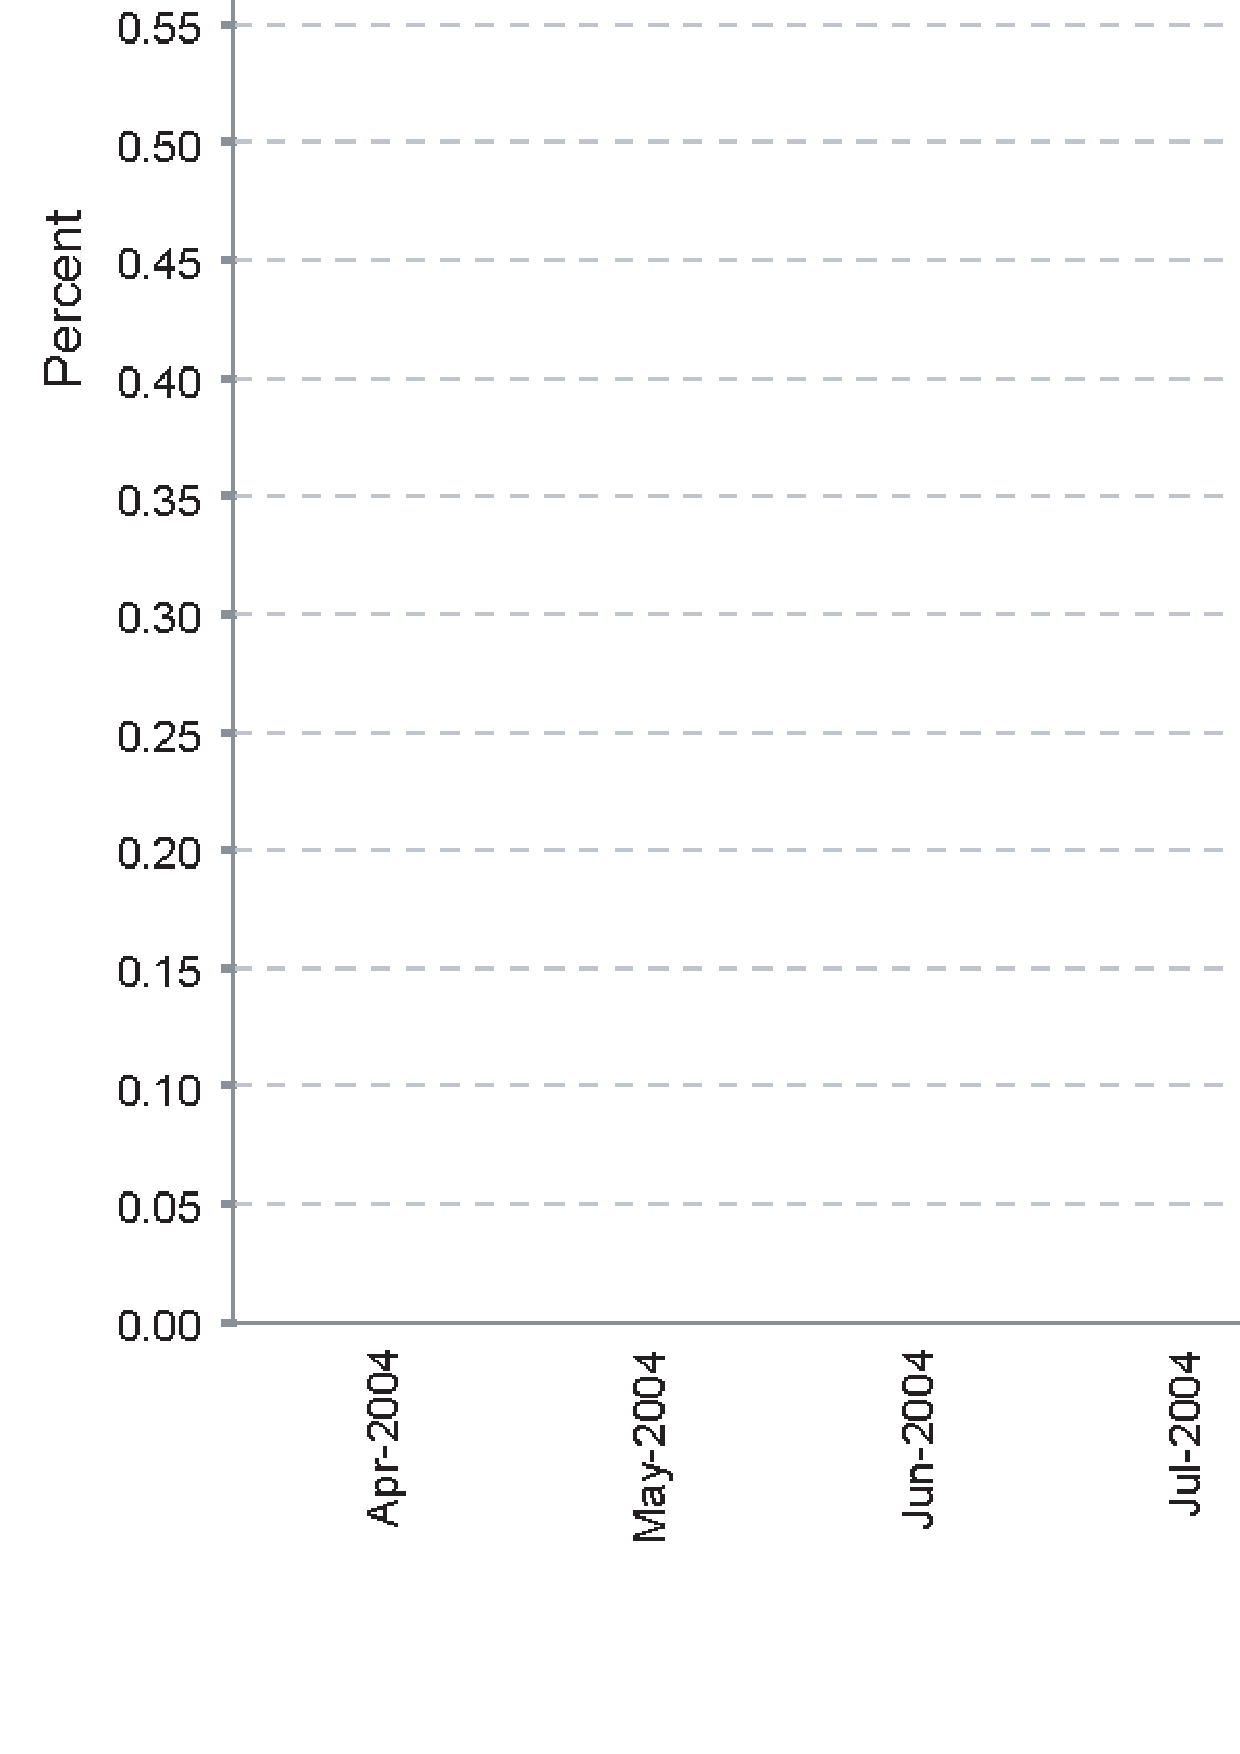
\includegraphics[height=0.90\textheight]{figures/TelemetryLanguageDemo}
%  \caption{Telemetry Language Demonstration} 
%  \label{fig:TelemetryLanguageDemo}
%\end{figure}
%
%\begin{verbatim}
%   streams CodeSizeStream(FilePattern) = {
%       "Lines of Code", 
%       JavaFileMetric("Sloc", FilePattern)
%   };
%
%   streams CoverageStream() = {
%       "Test Coverage", 
%       JavaCoverage("NumOfCoveredMethods")
%       / (JavaCoverage("NumOfCoveredMethods")
%          + JavaCoverage("NumOfUncoveredMethods"))
%   };
%
%   chart CodeSizeChart() = {
%       "Code Size", "Lines", 
%       CodeSizeStream("**"), CodeSizeStream("**/Test*.java")
%   };
%
%   chart CoverageChart() = {
%       "Coverage", "Percent", 
%       CoverageStream()
%   };
%
%   report MyReport() = {
%       "Test Process", 
%       CodeSizeChart(), CoverageChart()
%   };
%
%   draw MyReport();
%\end{verbatim}













%%%%%%%%%%%%%%%%%%%%%%%%%%%%%%%%%%%%%%%%%%%%%%%%%%%%%%%%%%%%%%%%%%%%%%%%%%%%%%%%%%%%%%%
%%%%%%%%%%%%%%%%%%%%%%%%%%%%%%%%%%%%%%%%%%%%%%%%%%%%%%%%%%%%%%%%%%%%%%%%%%%%%%%%%%%%%%%

\section{Telemetry-based Project Management and Process Improvement} 
\label{Telemetry:Process}


%Software project telemetry works seamlessly with the existing GQM paradigm and maturity-based frameworks to improve the capability of software development organizations by supplementing them with an explicit and practical framework for metrics collection and analysis:
%
%\begin{itemize}
%	\item \textit{The GQM paradigm} is used to generate high level organizational goals, and questions that need to be answered in order to reach the goals. Examples of the questions include: \textit{How much time are we spending on software development? How much time are we expending on testing software? What types of errors and changes are typical on our projects? Does test coverage affect defect rate?} These questions determine the set of telemetry streams we wish to monitor. The desired telemetry streams, in turn, determine what software metrics need to be collected and what kind of sensors need to be used.
%	
%	\item \textit{Process maturity} determines the visibility of software development activities in an organization. It determines what software metrics we can collect and analyze in a meaningful way. A measurement program, no matter how well it is implemented, can only measure what is visible in the process. For example, one may wish to measure software defects and study the relationship between defects and other attributes of the development process. However, if the software organization's maturity level is low, such as at CMM level 1, then it is almost certain that there is no defect tracking mechanism in place, and thus impossible to measure defects. Only when the process gets mature and defects are tracked can the measurement be taken. When the software organization reaches even higher level of maturity, more information about the defects are recorded, such as the type of defects, the attributes of the code associated with the defects, the cost of fixing the defects, etc. The process maturity sets a feasibility boundary of software metrics.
%	
%	\item \textit{Software project telemetry} provides an explicit and framework for software measurement. It offers practical guideline for metrics collection, analysis, and process improvement hypothesis validation.
%	
%\end{itemize}
%
%
%Together, they provide a meaningful context for software organizations to carry out process improvement programs.

Basic steps of telemetry-based process improvement are illustrated in Figure \ref{fig:TelemetryBasedProcessImprovement}. It involves cycles of problem detection, process improvement hypothesis generation, process change implementation, hypothesis validation, and impact analysis.

\begin{figure}[p]
  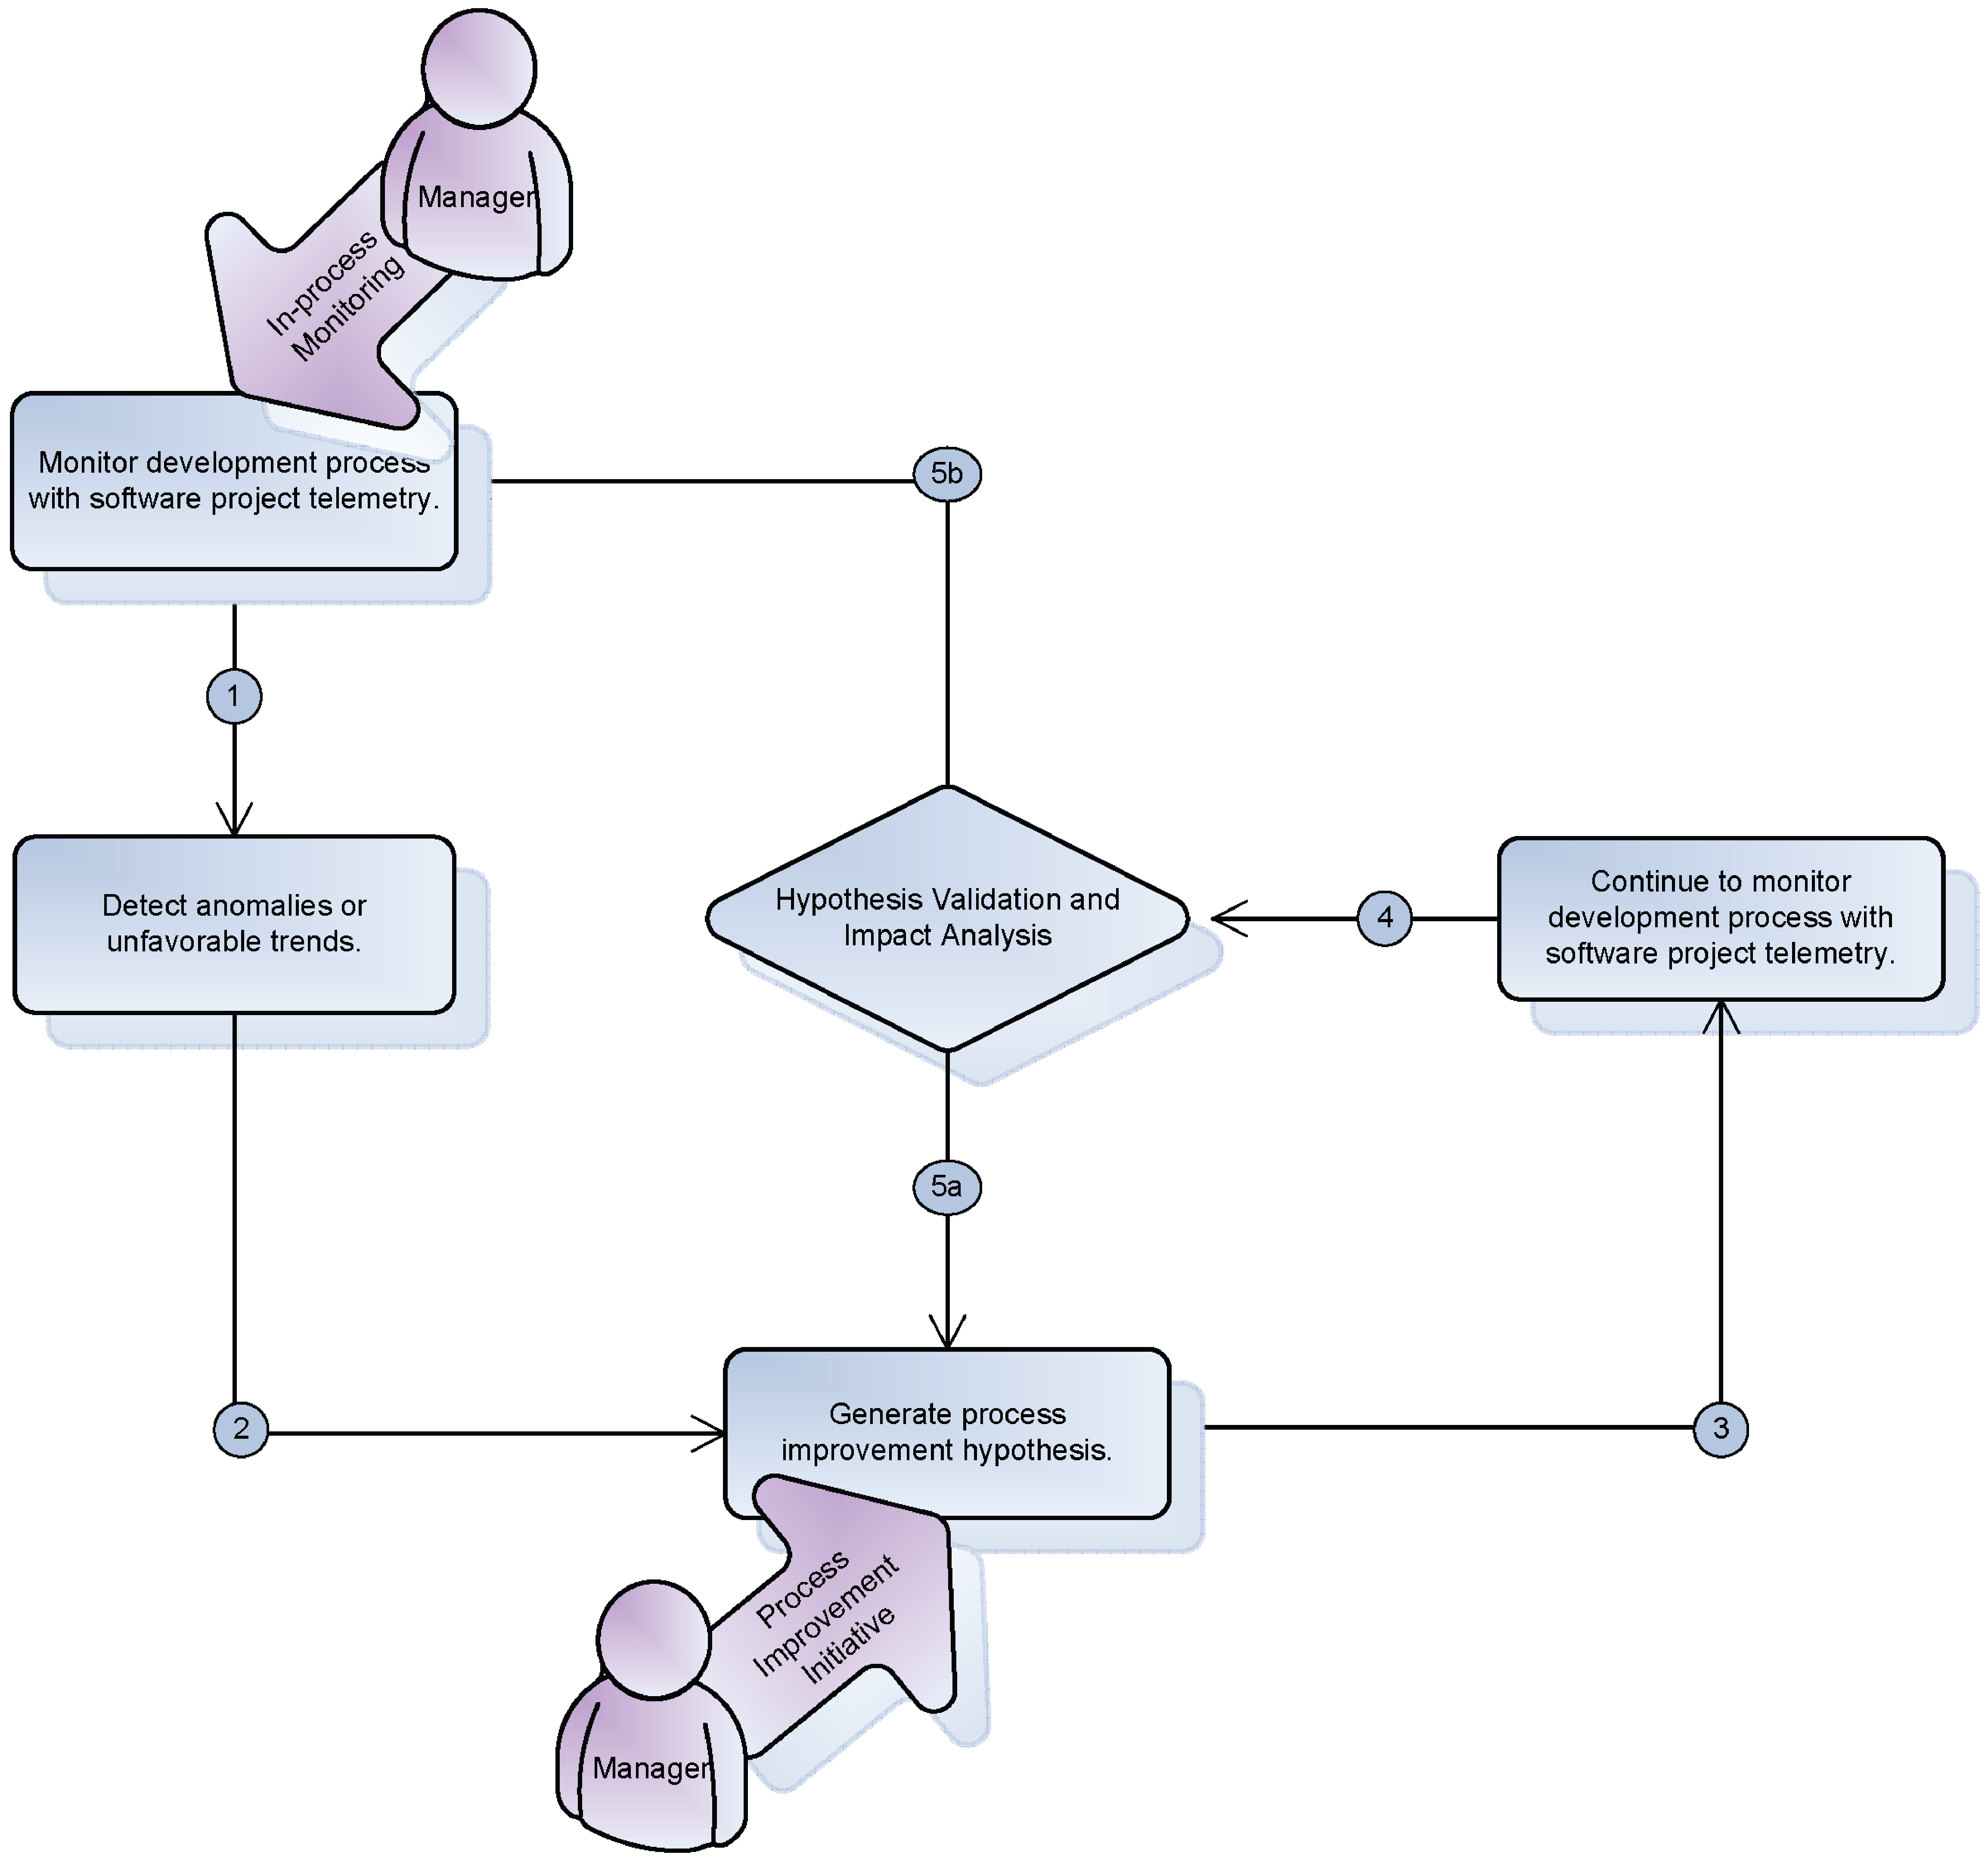
\includegraphics[width=1.00\textwidth]{figures/TelemetryProcess}
  \caption{Telemetry-based Process Improvement} 
  \label{fig:TelemetryBasedProcessImprovement}
\end{figure}

%The knowledge repository is at the core of telemetry-based process improvement programs. It contains the knowledge of useful telemetry streams, charts, reports, and the conditions under which they are most effective. The streams, charts, and reports are used to monitor, control, and improve software development process. 
%Some knowledge may be valid in general. However nothing guarantees that the knowledge that is valid and useful in one context and for some specified goal is as valid and useful for another context and goal. 

Following \cite{Hetzel:1993}, a software organization is recommended to collect a basic set of metrics, such as code size, test coverage, and build results, for every project at all time. This basic set of metrics can generate a basic set of telemetry streams which provide insights into the current software products, as well as a base line for the current development process.

Software project telemetry operates primarily in two modes: (1) in-process project monitoring mode, and (2) process improvement mode. The two modes are closely related, and sometimes indistinguishable in practical project management. However, I am trying to keep them separated here in order to make the concept clear. 


The steps for in-process project monitoring mode start from the upper arrow in Figure \ref{fig:TelemetryBasedProcessImprovement}. Telemetry streams are monitored for anomalies and unfavorable trends. If anomalies or unfavorable trends are detected, then the project manager must investigate the cause. Multiple telemetry streams, representing different perspectives on development process, are used to detect correlations. For example, one might find that complexity telemetry values are increasing as well as defect density. Since telemetry streams consist of time-stamped events, the sequence of detected changes in different telemetry streams might help the project manager generate hypothesis about the causal relationship and corrective measurements for process improvement. For example, one might identify code complexity as the likely cause for high defect density. Once the process improvement hypothesis is generated, the project manager tries corrective action such as simplifying over-complex modules, and continues to monitor telemetry streams in order to check whether the action results in a decrease in defect density. It might be necessary to monitor new telemetry streams embedded with the hypothesis at this stage. One can also monitor other telemetry streams to check if such corrective action has unintended side-effects (impact analysis). If the hypothesis is correct, it will be validated by telemetry streams. If telemetry streams indicate otherwise, then there must be other reasons that cause high defect density, and the project manager must try other corrective measures. The knowledge acquired through such exercise can be generalized into rules. The rules are stored in the software organization's knowledge repository, and used in the next project.

The steps for process improvement mode follow the same loop as the steps for in-process project monitoring mode. The only difference is that they start from the lower arrow in Figure \ref{fig:TelemetryBasedProcessImprovement}, and implementation of process improvement measures does  not have to wait until anomalies or unfavorable trends are detected in telemetry streams. 



%Telemetry-based project management and process improvement follow sound scientific discipline.
%In a sound engineering approach, we need to determine:
%\begin{itemize}
%	\item whether the evidence is sufficient to draw reliable conclusions (e.g. is the evidence only anecdotal or do statistical procedures such as the test of hypotheses confirm the hypothesis?)
%	\item the absence of other influencing factors (e.g. has maintainability improved because of the adoption of object-oriented programming or because of the improvement in the education of programmers or the adoption of CASE tools?)
%	\item the extent of the impact of the influencing attributes on the influenced attribute (e.g. does module cohesion influence software maintainability more than module coupling does? What is the impact of a variation in module coupling on maintainability?)
%\end{itemize}









%%%%%%%%%%%%%%%%%%%%%%%%%%%%%%%%%%%%%%%%%%%%%%%%%%%%%%%%%%%%%%%%%%%%%%%%%%%%%%%%%%%%%%%
%
%      This section is commented out!
%
%      Could use this one
%http://hackystat.ics.hawaii.edu/hackystat/docbook/ch05s02.html
%
%%%%%%%%%%%%%%%%%%%%%%%%%%%%%%%%%%%%%%%%%%%%%%%%%%%%%%%%%%%%%%%%%%%%%%%%%%%%%%%%%%%%%%%
\begin{comment}
\section{A Simple Example}
\label{Telemetry:Example}

\textcolor{red}{[Please ignore this section.]} [I plan to change this section to use an example with lots of screen shot from Hackystat, similar to the one available at
http://hackystat.\-ics.\-hawaii.\-edu/\-hackystat/\-docbook/\-ch05s02.html.]

This is a fictional scenario to illustrate the working of telemetry-based process improvement approach. The story unfolds in \textit{HPC Soft}, a startup company developing software called \textit{Stack Hack}, which has the potential to increase software developer productivity on high performance super computers by 10 times. The manager \textit{Philip} uses \textit{software project telemetry} to manage the project.

In this scenario, a project manager uses sensors to collect software metrics and generates telemetry streams. Suppose there are two telemetry streams in front of our manager: one representing defect density, and the other representing unit test coverage. Our manager finds that as the project goes on, the defect density goes up and at the same time the unit test coverage goes down. The manager knows that this is bad because the project might fail if the trend continues.

Our manager investigates and finds out that most developers do not follow any methodology when writing test cases. When the project becomes more complex, it's increasingly difficulty to test the system thoroughly by writing test cases in ad-hoc fashion. Low test coverage causes more bugs to escape from developers. If everybody can follow test driven design principle by writing test cases before implementing any features and modifying code only if test fails, test coverage will increase. Higher test coverage will result in more bugs being detected by developers and thus lowering defect density.

Convinced by his hypothesis, our manager talks to his developers and convinces them of the advantages of test driven design. After everyone has adopted test driven design principle, our manager collects more data to update the telemetry streams and check whether switching to test driven design does indeed increase test coverage and lowers defect density as he has expected.

If everything does not happen as expected (assuming that developers are following test driven design principles), it means that our manager's hypothesis (ad-hoc testing causes lower coverage as system becomes more complex, which in turn causes higher defect density) is incorrect. Either test driven design does not increase coverage, or higher coverage does not result in lower density. Either way our manager needs to collect more metrics, generate more telemetry streams to find out the true cause of the problem. 

However, on the other hand, if our manager's hypothesis is correct, then it will be confirmed by the updated telemetry streams. In this case, our manager might want to check other telemetry streams to see whether adopting test driven design has any unintended side effect on his development team. For example, what is the effect of test driven design on developer productivity? Will it lower productivity? If it does, is it temporary or permanent? A new telemetry stream capturing team productivity can answer all these questions.

As the example illustrates, the general style of telemetry-based software project management involves cycles of:
\begin{itemize}
  \item Problem detection: Is there any anomaly in telemetry streams, or do they exhibit undesirable trend?
  \item Hypothesis generation: What is the possible causes for the problem, and how do I correct them?
  \item Hypothesis testing: Does the problem go away after corrective measures are implemented?
  \item Impact analysis: Is there any unintended side effects caused by the corrective measures?
\end{itemize}
The cycle continues until the project is completed.
\end{comment}





%%%%%%%%%%%%%%%%%%%%%%%%%%%%%%%%%%%%%%%%%%%%%%%%%%%%%%%%%%%%%%%%%%%%%%%%%%%%%%%%%%%%%%%
%%%%%%%%%%%%%%%%%%%%%%%%%%%%%%%%%%%%%%%%%%%%%%%%%%%%%%%%%%%%%%%%%%%%%%%%%%%%%%%%%%%%%%%

\section{Summary}
\label{Telemetry:Conclusion}

Software project telemetry includes both (1) highly automated measurement machinery for metrics collection and analysis, and (2) a methodology for in-process, empirically-guided software development process problem detection and diagnosis. It overcomes many of the difficulties in existing approaches to software measurement and process improvement. The next chapter compares and contrasts software project telemetry to those approaches.






%%%%%%%%%%%%%%%%%%%%%%%%%%%%%%%%%%%%%%%%%%%%%%%%%%%%%%%%%%%%%%%%%%%%%%%%%%%%%%%%%%%%%%%
%%%%%%%%%%%%%%%%%%%%%%%%%%%%%%%%%%%%%%%%%%%%%%%%%%%%%%%%%%%%%%%%%%%%%%%%%%%%%%%%%%%%%%%

%\section{Discussion}
%
%\subsection{Automatic and Unobtrusive Metrics Collection}
%
%Software project telemetry is based on the idea of sensor-based automatic and unobtrusive metrics collection. It solves measurement dysfunction problem by removing the overhead of software product and process data collection completely from developers.
%
%At the same time, sensor-based metrics collection lowers total cost of the measurement program drastically. Automated data collection makes it possible for software organizations to apply measurement to all development activities on a continual basis. The increased measurement capability allows a more comprehensive quantitative view of an organization's process status.  
%
%\subsection{Flexible and Robust Analysis}
%
%Software project telemetry analysis is flexible. The types of metrics that can be collected is only constrained by the available of sensors. It is always possible to write a new sensor to collect new type of software metrics, and there is virtually limitless possibilities of generating telemetry streams by filtering, combining, and aggregating the metrics. 
%
%Software project telemetry analysis is robust too. There is no requirement for complete set of telemetry data. While complete set of telemetry data provides best support for project management, the telemetry analysis can still provide value even if sensor data occasionally become unavailable.
%
%\subsection{Exploratory Project Management}
%
%Software engineering is a very human-intensive discipline. Software development is, to a larger extent, a social phenomenon occurring in a complex and changing environment. We often do not have a good understanding of the attributes of software products and development process we are trying to measure, especially the relationships between them. 
%
%Software project telemetry supports an exploratory approach to project decision-making. Telemetry streams can be designed with embedded process improvement hypothesis, which can be validated by observing the changes in those telemetry streams.   
%
%\subsection{In-process Monitoring and Control}
%
%Telemetry analysis provides representation of current project status and how it is changing over time. Project management based on software project telemetry does not require historical project database which is often necessary in prediction model based approaches. 
%
%The simultaneous display of multiple telemetry streams and how they change over the same period of time allows opportunistic analysis --- the emergent knowledge that one state variable correlates with another in the context of the current project.







% The flexibility of generating telemetry streams: can help build and validate hypotheses and increase the body of knowledge about software engineering. This body of knowledge can be used to understand, monitor, control, improve software process and products.

% Telemetry streams contains time-stamped events, which can be used to determine the sequence of events. Though it is not sufficient to determine the causal relationship, it helps users greatly to generate a hypothesis. Telemetry streams can then be designed by embedding the hypothesis, and monitored to either confirm or reject the hypothesis. 

%Software project telemetry streams are made from time-stamped metrics, they display the history of software development process change. By focusing on change detection and change control, software organizations can reduce variation in their software development processes and increase their capabilities. 






% Telemetry streams can be at product, process, organizational level. There is a paper.



%%%%%%%%%%%%%%%%%%%%%%%%%%%%%%%%%%%%%%%%%%%%%%%%%%%%%%%%%%%%%%%%%%%%%%%%%%%%%%%%%%%%%%%
%%%%%%%%%%%%%%%%%%%%%%%%%%%%%%%%%%%%%%%%%%%%%%%%%%%%%%%%%%%%%%%%%%%%%%%%%%%%%%%%%%%%%%%

%\section{Assessment}

%Success factors can be identified for implementing metrics programs based on experiences reported in the literature. (Hall and Fenton 1997, Grady 1992, Pfleeger 1993). 
%\begin{itemize}
%	\item The metrics program must obtain acceptance from the developers, and they must be convinced that the metrics program is useful and not used against them.
%	\item The metrics program should be incrementally implemented and constantly improved.
%\end{itemize}
%
%Above are high level goals, which can be translated to low level goals.
%
%\begin{itemize}
%  \item Low TCO (1. affordable to individual developers, small teams, small organizations, which do not have dedicated process improvement team. 2. Show me the benefit before I will implement the metrics program. But if you don't try the metrics program, how can you see the benefit. Low TCO helps break the vicious circle.).
%	\item Data Collection - Elimination of metrics collection overhead
%	\item Data Analysis - Explorative analysis
%	
%	
%	\item Robust (graceful to handle missing data points) 
%	\item Flexible but useful analysis (agile), Support incremental metrics program improvement
%	
%	
%	\item A base set of basic metrics should always be collected (to stimulate hypothesis generation and process improvement).
%	\item Support hypothesis validation (telemetry streams can be designed so that they embed process improvement hypothesis).
%	\item Robustness of analysis is really important. We have to assume that metrics collections are error prone. Data will be missing or distorted. The data verification mechanism should be built into the system to check for data anomalies. Even if data is collected automatically, sensor may always malfunction.
%	\item Measurement data should be presented in a manner that make it easy to communicate and assimilate the information it contains. One of the most effective ways is to present the information graphically. Good graphics can greatly increase our ability to compare and contrast data, to identify trends, patterns and outliers.
%	\item Check 04-11, see what Philip says.
%\end{itemize}
%
%\textit{Success Factors Adhered to in Telemetry-base Process Improvement Approach}

%Several authors have identified a list of success factors for implementing measurement programs based on experiences reported in the literature. Success factors listed by Hall and Fenton 1997 is used below to assess software project telemetry approach.
%
%\textcolor{red}{[Fill the table]}
%
% Other literatures are: Grady 1992, Pfleeger 1993, Jeffery and Berry 1993, Rifkin and Cox 1991
%
%\begin{table}[tbp]
%	\centering
%		\begin{tabular}{|p{0.60\textwidth}|p{0.30\textwidth}|} 
%		  \hline
%			\textbf{Success Factors} & \textbf{Evaluation} \\
%			\hline 
%			\textit{Incremental implementation.} & Yes. \\
%			\hline
%			\textit{Well-planned metrics framework.} & -. \\
%			\hline
%			\textit{Use of existing metrics material.} & -. \\
%			\hline
%			\textit{Involvement of developers during implementation.} & Yes. Telemetry streams are not hidden in database guarded by the software quality improvement group. Instead, they are visible to all developers of the project. \\
%			\hline
%			\textit{Measurement process transparent to developers.} & Yes. Sensors are used to collect metrics automatically and unobtrusively. \\
%			\hline
%			\textit{Usefulness of metrics data.} & -. \\
%			\hline
%			\textit{Feedback to developers.} & -. \\
%			\hline
%			\textit{Ensure that data is seen to have integrity.} & -. \\
%			\hline
%			\textit{Measurement data is used and seen to be used.} & -. \\
%			\hline
%			\textit{Commitment from project managers secured.} & -. \\
%			\hline
%			\textit{Use automated data collection tools.} & -. \\
%			\hline
%			\textit{Constantly improving the measurement program.} & -. \\
%			\hline
%			\textit{Internal metrics champions were used to manage the program.} & -. \\
%			\hline
%			\textit{Use of external metrics gurus.} & -. \\
%			\hline
%			\textit{Provision of training for practitioner.} & -. \\
%			\hline
%		\end{tabular}
%	\caption{Metrics Program Success Factors}
%	\label{table:Metrics-Success-Factors}
%\end{table}
